\documentclass[12pt]{article}\pagestyle{myheadings}
\usepackage{graphicx}
\usepackage{placeins}

\textwidth 7.0 truein
\oddsidemargin -0.25in   %left-hand edge
\evensidemargin -0.5 truein  %right-hand edge
\topmargin -0.85in      %top of paper to top of head, pulls whole unit
\textheight 9.5in

%Enter your last name, the portfolio problem number, and the draft number.
\title{Homework 2 \\ Chaotic Dynamics - CSCI 4446}
\author{Denis Kazakov}
\date{January 24, 2015}


\usepackage{amsmath,amssymb,amsthm,amsfonts,graphicx}
%The following commands allow us to typeset theorems, propositions, definitions, etc.
\theoremstyle{plain}
\newtheorem{theorem}{Theorem}
\newtheorem{lemma}[theorem]{Lemma}
\newtheorem{corollary}[theorem]{Corollary}
\newtheorem{proposition}[theorem]{Proposition}
\newtheorem*{definition}{Definition}

\renewcommand{\qedsymbol}{\ensuremath{\blacksquare}}
\newcommand{\N}{\mathbb{N}}
\newcommand{\Z}{\mathbb{Z}}
\newcommand{\Q}{\mathbb{Q}}
\newcommand{\R}{\mathbb{R}}
\newcommand{\C}{\mathbb{C}} 

\begin{document}
\maketitle


\section{Problem 1}

\begin{figure}[h!]
\centering
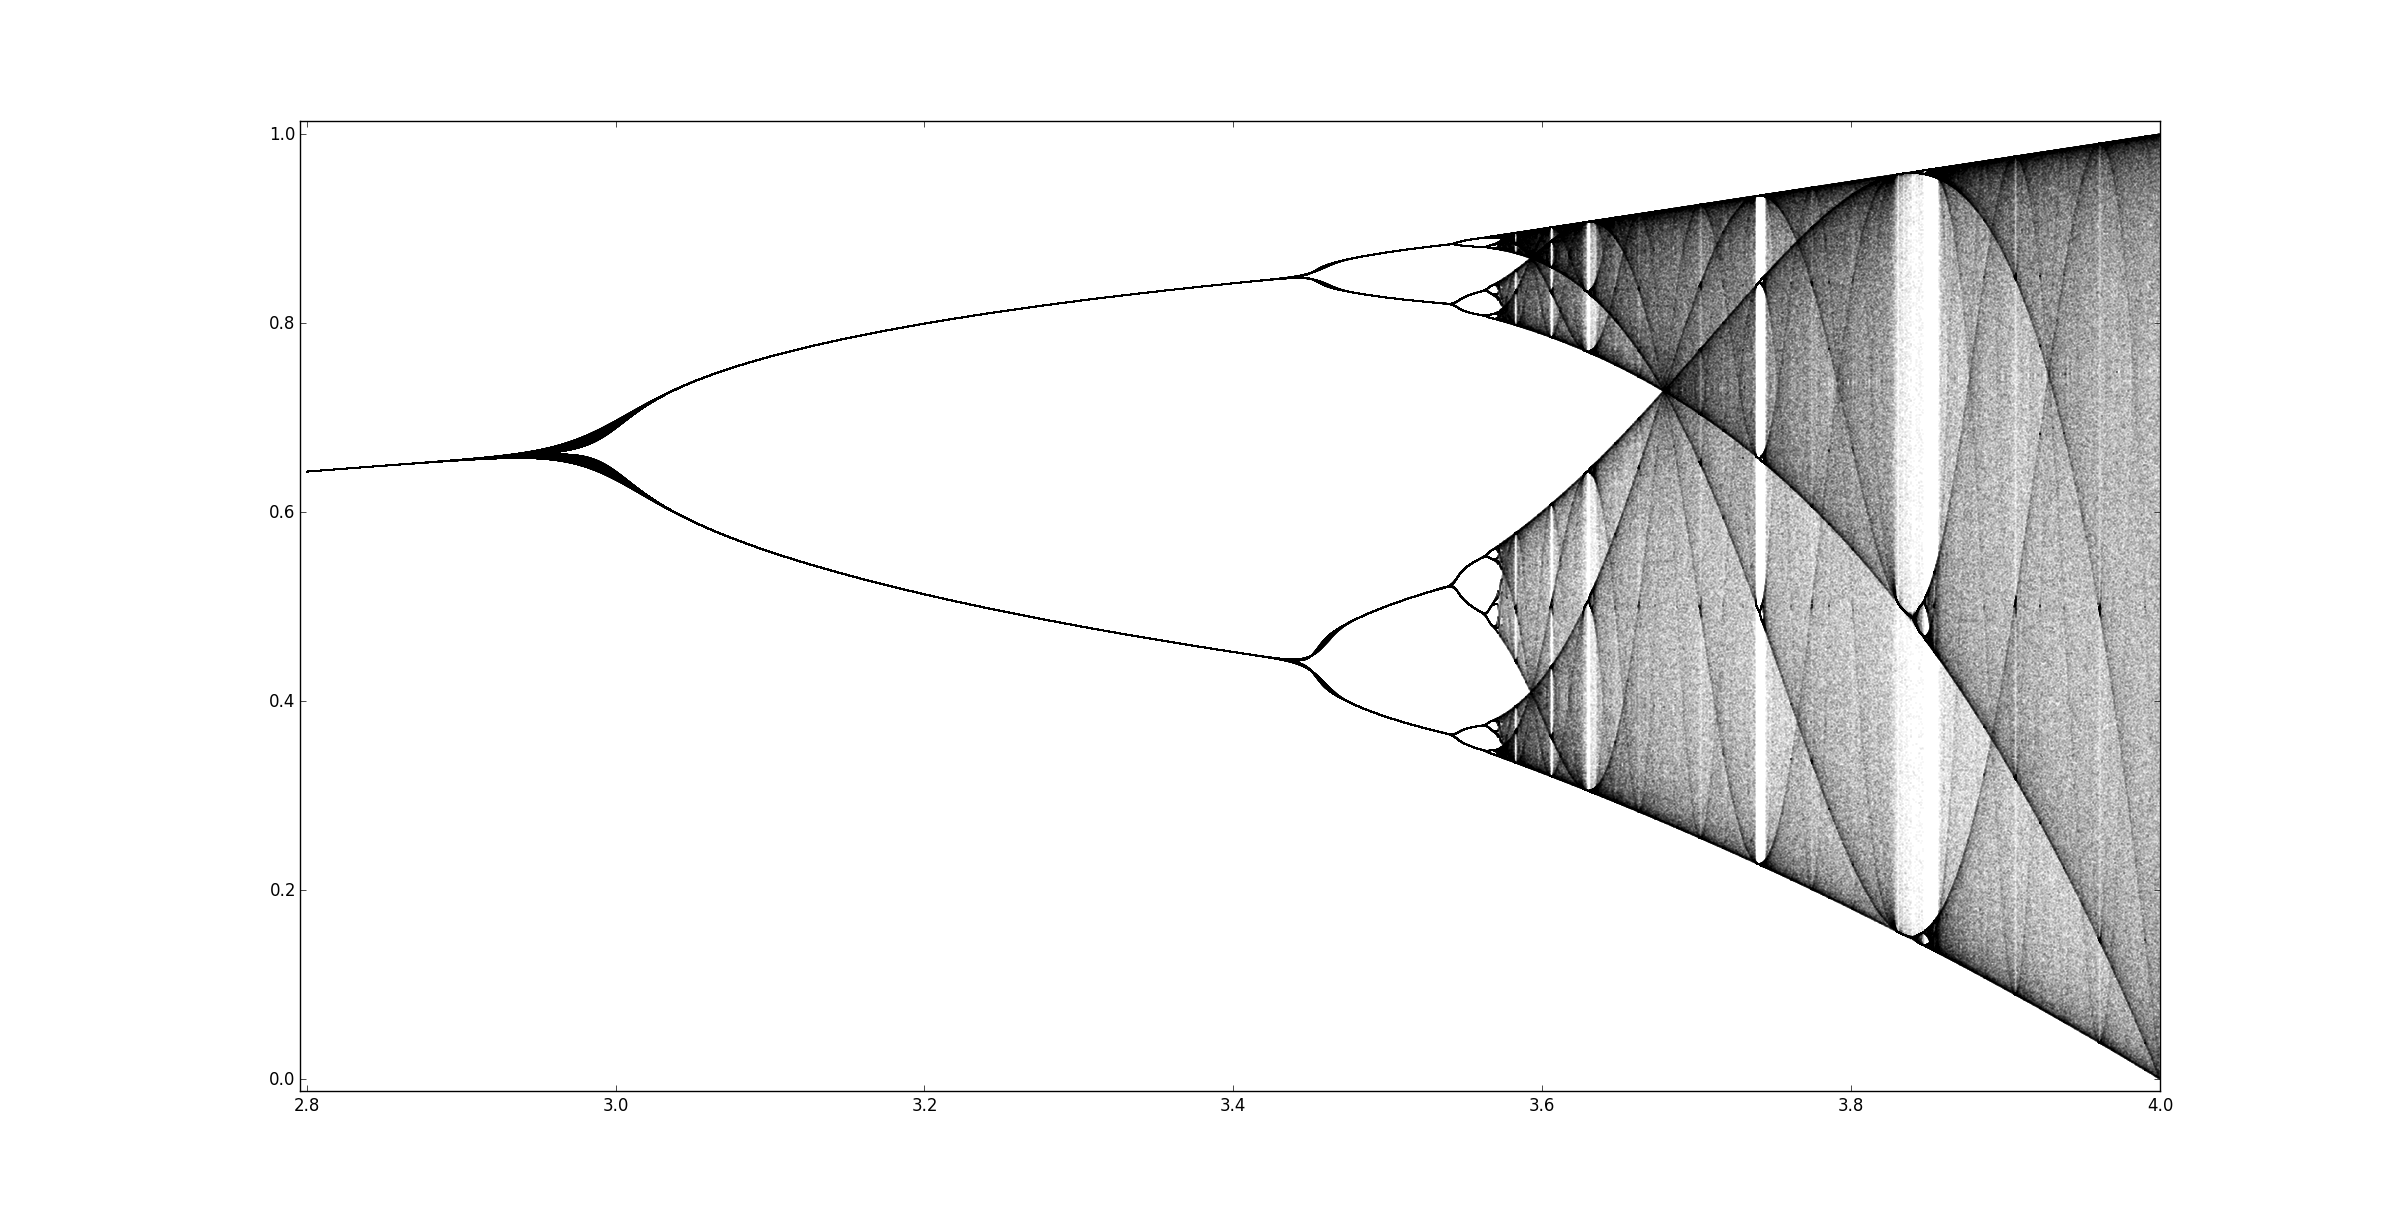
\includegraphics[scale=.3]{nice_bifurcations}
\caption{Bifurcation plot for $2.8 < R < 4$, l = 50 , m = 100, $x_0$ = 0.2}
\label{fig:my_label}
\end{figure}


\section{Problem 2}
Estimating Feigenbaum number:
Let's come up with a simple moment generating function for each value of R:

$$mgf(R) = \sum_{i=1}^{m-l} \exp^{X[i]}$$, where $X[i]$ is i'th element of the iteration points array for given R value. \\

If we plot such moment generating function against R, we get a simple plot showing qualitative changes in our bifurcation plot as R changes:\\

\begin{figure}[h!]
\centering
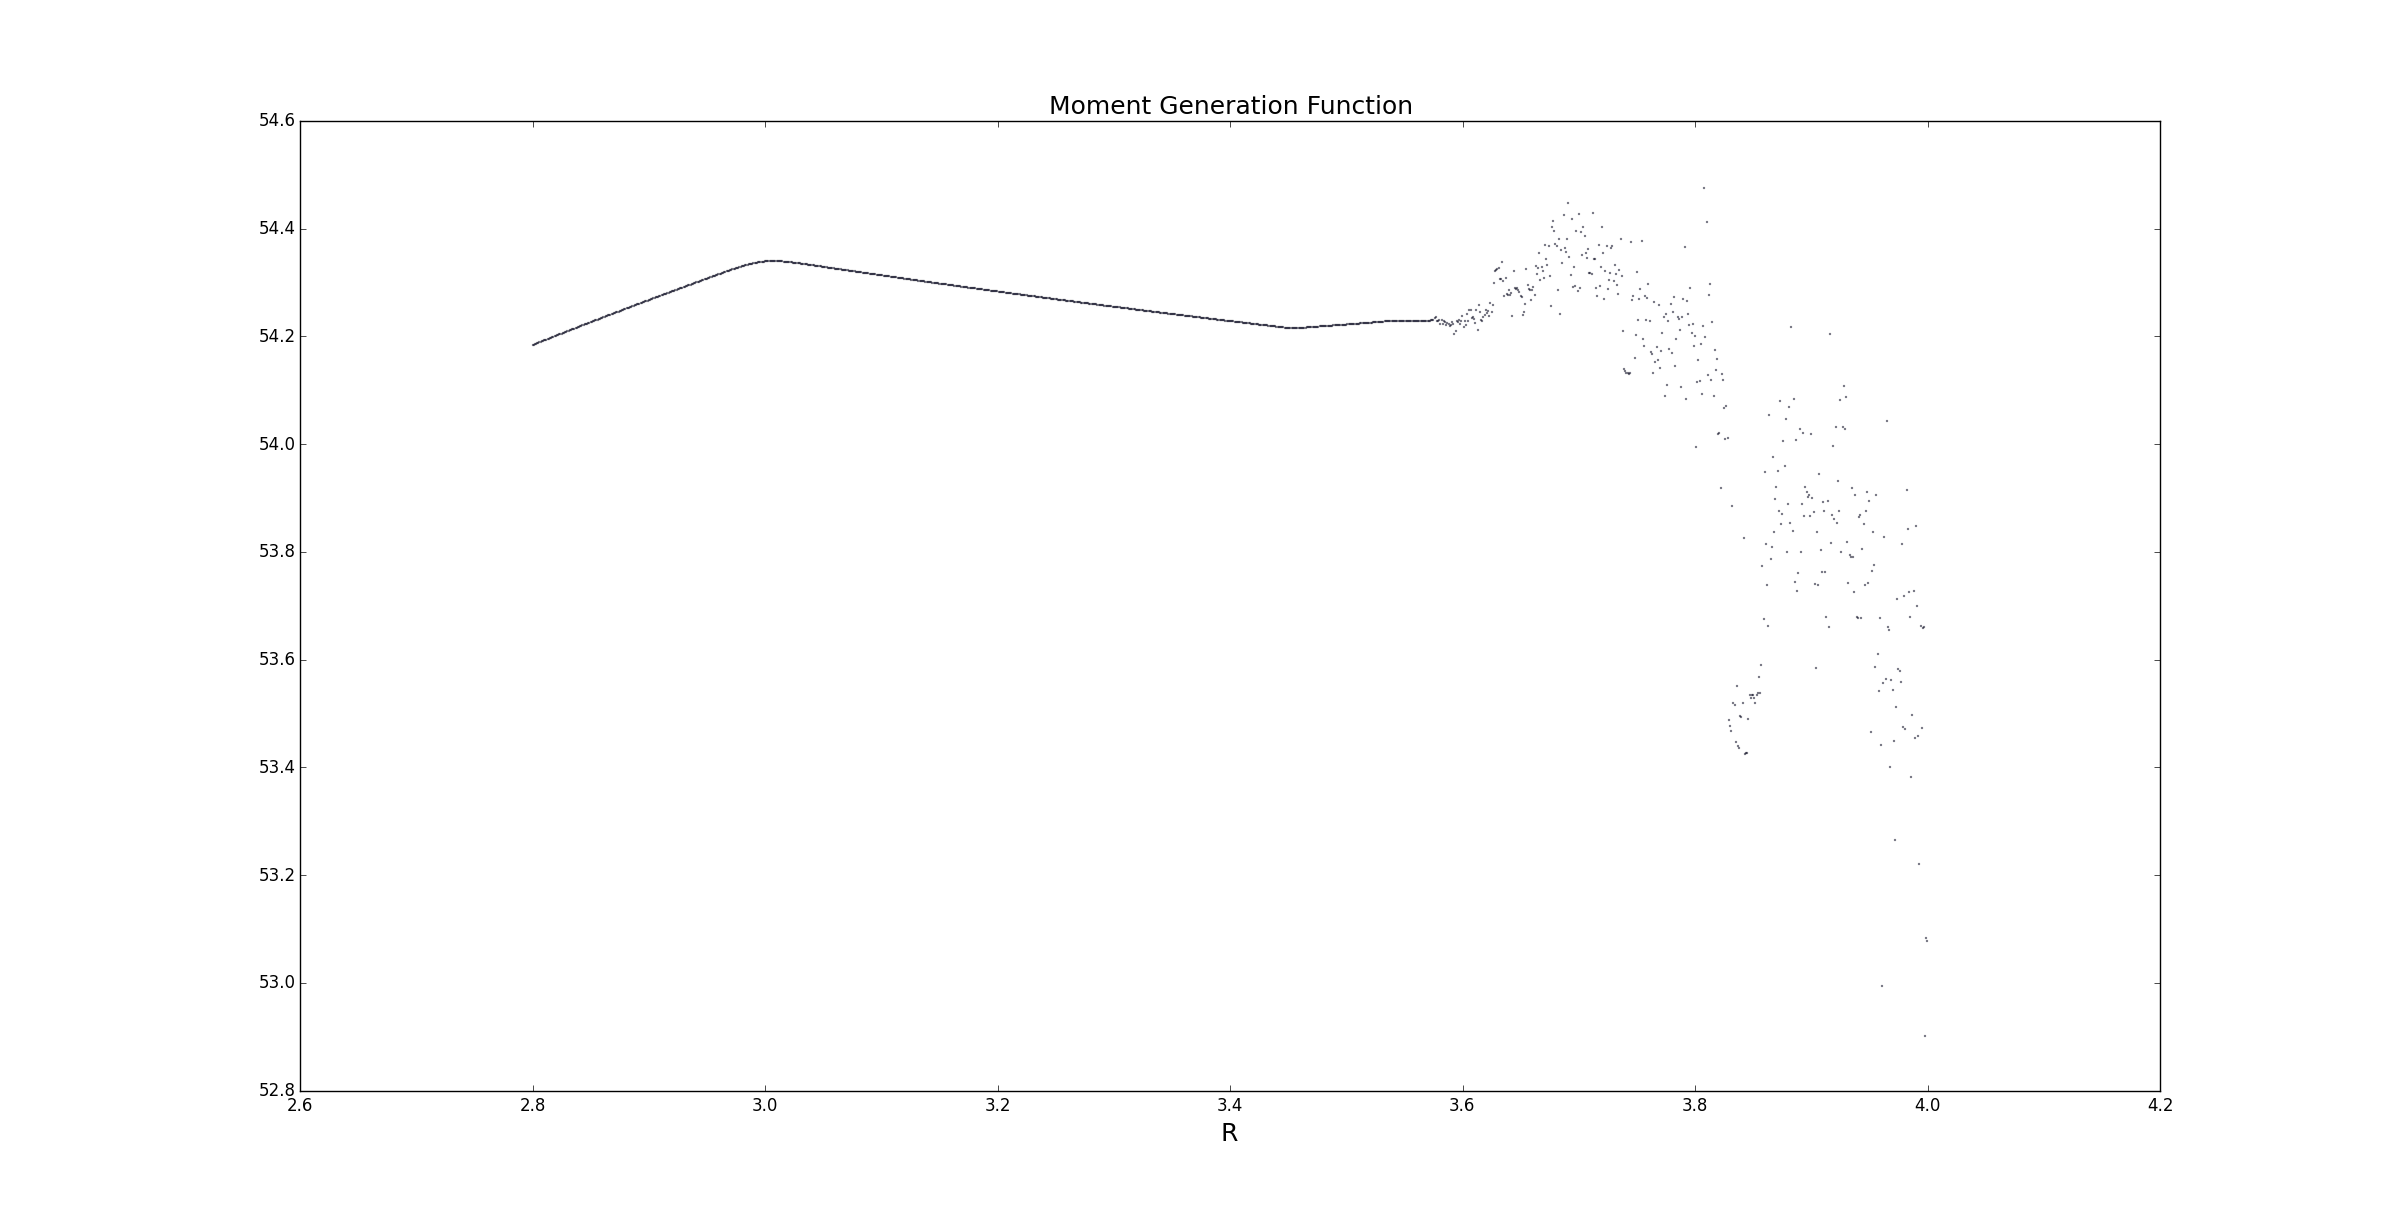
\includegraphics[scale=.3]{moment_gen_2}
\caption{Moment Generating Function plot - $mgf(R)$. R values for which slope of $mgf(R)$ changes are the bifurcation points. }
\label{fig:my_label}
\end{figure}

In the $mgf(R)$ function, it's easy to spot the sudden changes in the slope of the function. Those changes imply qualitative change in the bifurcation plot. It's easy to see how those points correspond to bifurcation points. 
From the $mgf(R)$ plot and further analysis of the bifurcation plot, we can identify the following bifurcation points: 
\begin{enumerate}
\item 2.94 - 2 periodic
\item 3.429 - 4 periodic
\item 3.54 - 8 periodic, $\frac{PreviousBifurcationLength}{CurrentBifurcationLength} = 4.40540540541$
\item 3.561 - 16 periodic, $\frac{PreviousBifurcationLength}{CurrentBifurcationLength} = 5.28571428571$
\end{enumerate}

Our estimate of Feigenbaum number then comes to the average of $4.8455598$, which is fairly close to the known $4.669$. 

\section{Problem 3}
Henon map:
$$x_{k+1} = y_{k} + 1 + \alpha x_{k}^2$$
$$y_{k+1} = \beta x_{k}$$

Since we now have 2 dimensional system, let's follow the same format as we did in problem 1 and plot only $x$ values iterations on the bifurcation map. 

\begin{figure}[h!]
\centering
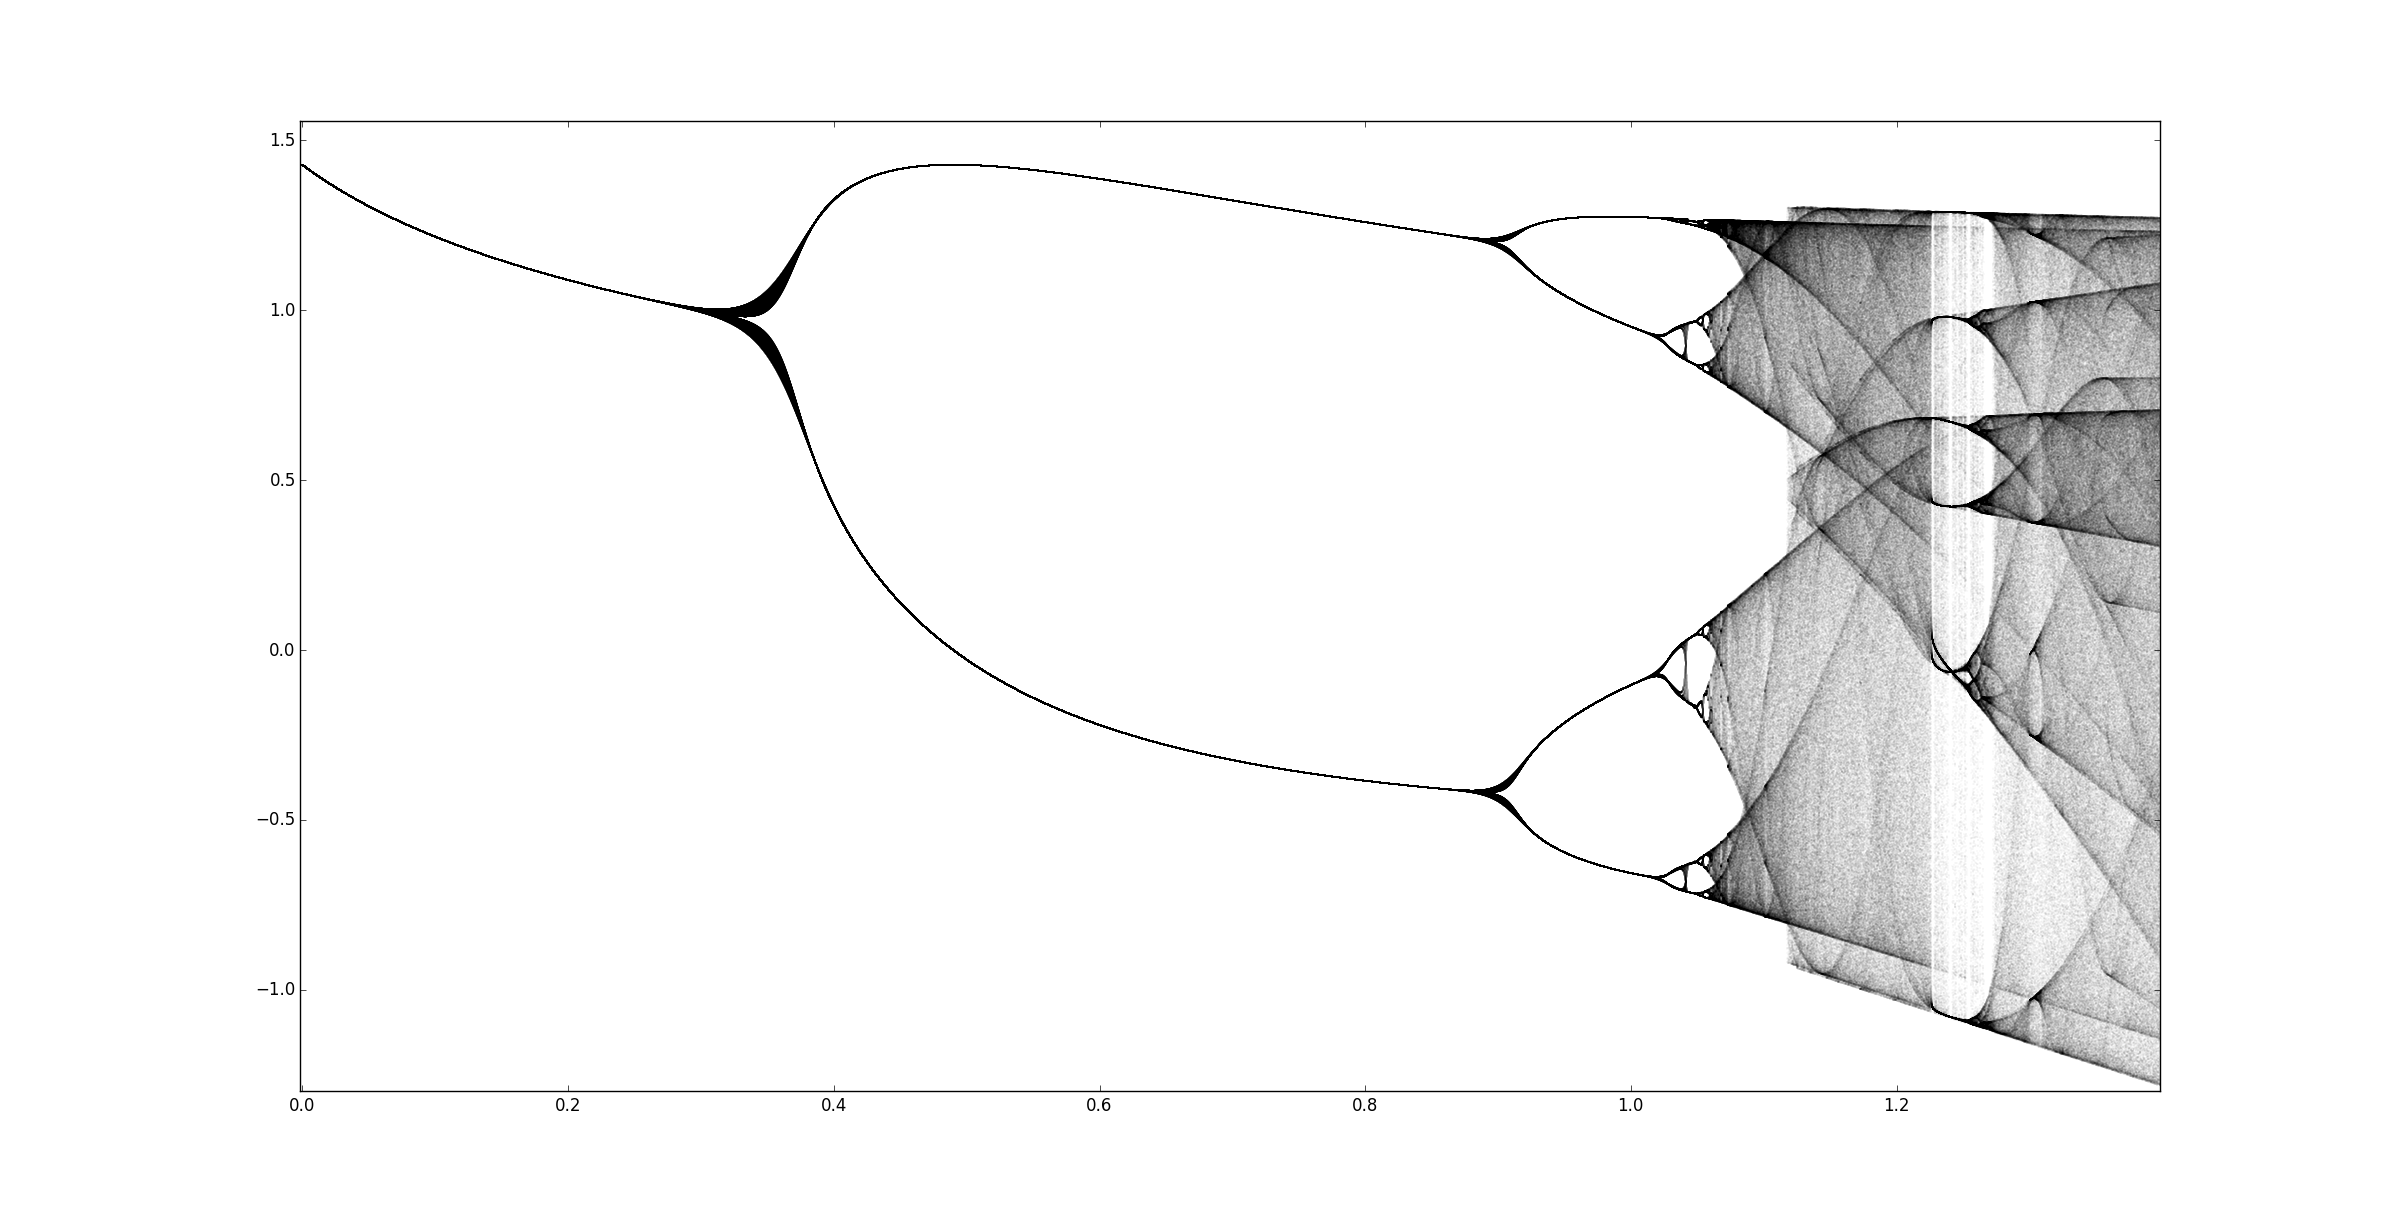
\includegraphics[scale=.3]{henon_bifurcations}
\caption{Bifurcation plot for x-dimension change of Henon map: $0 < \alpha < 1.4$, $\beta = 0.3$, $x_0 = 0.2$, $y_0 = 0.2$, l = 50 , m = 100}
\label{fig:my_label}
\end{figure}

Let's make a moment generating function plot just like we did for the rabbit population model:

\begin{figure}[h!]
\centering
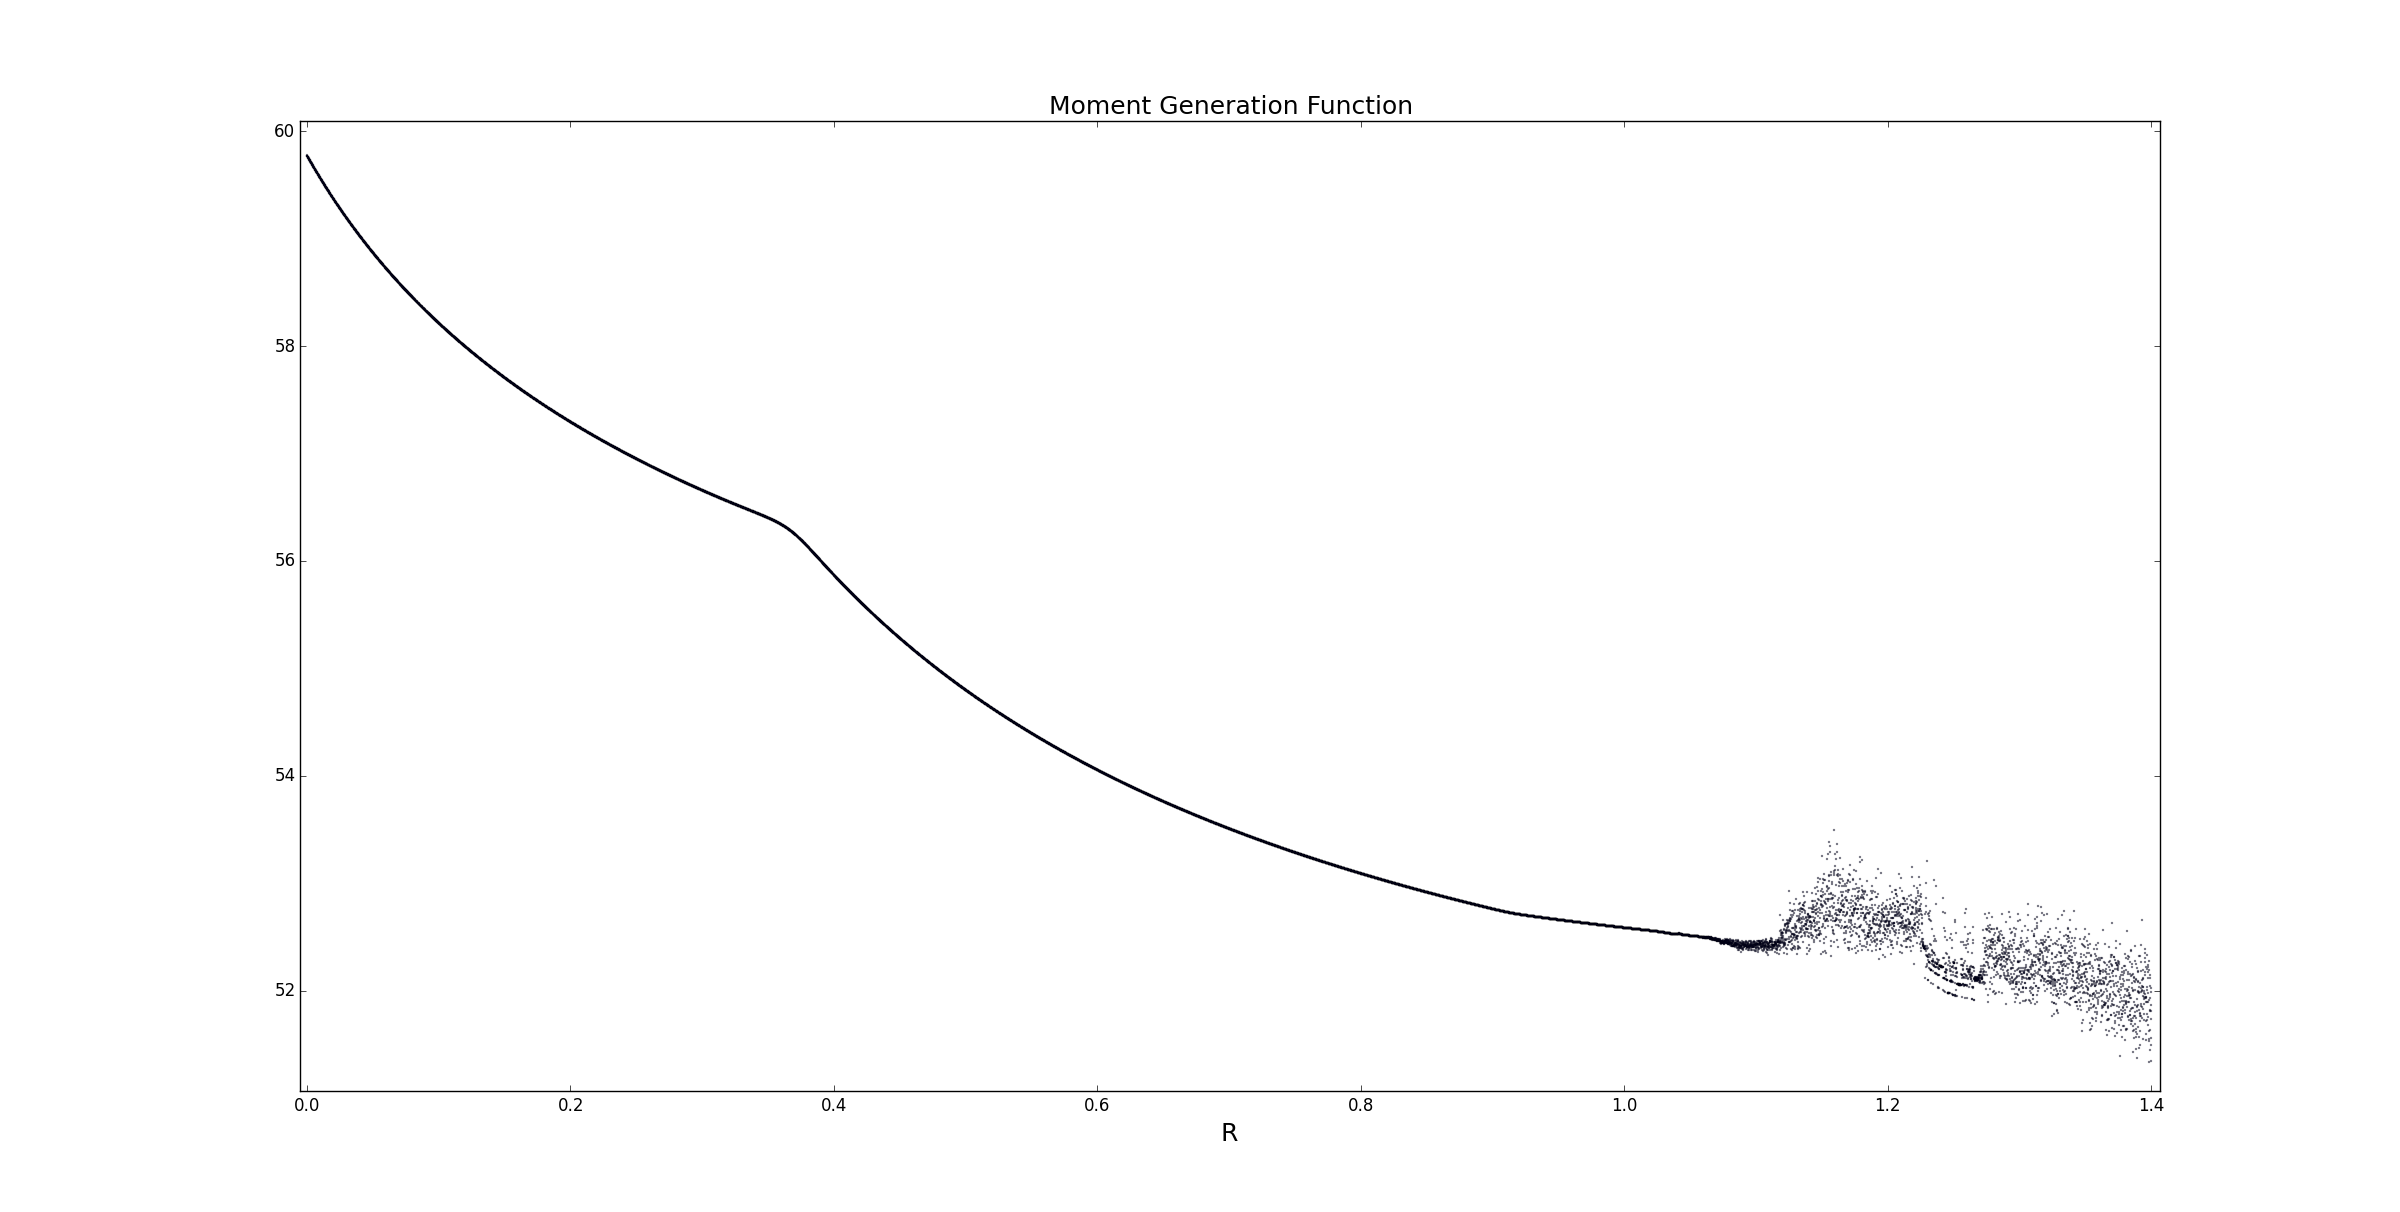
\includegraphics[scale=.3]{moment_gen_henon}
\caption{Moment Generating Function plot - $mgf(R)$ for Henon map.}
\label{fig:my_label}
\end{figure}

From the plot and further analysis of the bifurcation plot, we can identify the following bifurcation points: 
\begin{enumerate}
\item 0.26 - 2 periodic
\item 0.880 - 4 periodic
\item 1.015 - 8 periodic, $\frac{PreviousBifurcationLength}{CurrentBifurcationLength} = 4.51851851852$
\item 1.0445 - 16 periodic, $\frac{PreviousBifurcationLength}{CurrentBifurcationLength} = 4.57627118644$
\end{enumerate}

Our estimate of Feigenbaum number then comes to the average of $4.54739485248 $, which is fairly close to the known $4.669$. 

\section{Problem 4}

The two Feigenbaum numbers ($4.8455598$ - rabbit growth, $4.54739485248$ - Henon map) are close to the known constant of $4.669$.\\
We are guaranteed a Feigenbaum number of $4.669$ for one-dimensional maps. However, we clearly observe the same pattern for the two-dimensional Henon Map, which makes us wonder what makes "chaos" behave so "predictably". 

\end{document}